Chapter \ref{ch:approach} has formalized the problem and put forward a novel framework for finding useful words, consisting of two major functionalities:
Vocabulary list generation, and vocabulary list evaluation.
The list evaluation approach, described in Section \ref{sec:experimental-setup-with-ai}, utilizes the performance of an AI model on an NLP task with a context-specific corpus as input as a proxy metric for language ability, in order to estimate how efficiently the vocabulary list may help a human language learner acquire competency.
The list generation approach, proposed in Section \ref{sec:list-generation}, additionally uses Explainable AI as a tool for analyzing the interaction of the AI model with the corpus to compile vocabulary lists that approach maximal efficiency.

In this chapter, we describe our implementation, especially of the list generation approach.
This is because the list evaluation method is used in Chapter \ref{ch:evaluation} as one among several metrics for evaluating the efficiency of vocabulary lists generated by the implementation in this chapter.
However, the evaluation with our approach uses the same AI models and Corpora as the list generation approach.

We first discuss the implementation of the list generation approach from a system design perspective in Section\ref{sec:data-pipeline}, describing how we generate lists of vocabulary, without elaborating on the interdependencies that arise between concrete NLP tasks, corpora, and XAI methods.
The choice of those three components in the system is then argued in the following sections, each of which features a section where we discuss desiderata of the specific component on the basis of our aim as stated in Section \ref{sec:formal-problem-statement}, followed by the selection of concrete components.
Finally, we return to the holistic perspective in Section \ref{sec:implementation-final}, where we present the complete implementation with all individual components integrated.

\section{Data Pipeline} \label{sec:data-pipeline}

This section gives a top-level overview of our implementation for the list generation approach described in Chapter \ref{ch:evaluation}.
As mentioned before, the main components of this approach are:

\begin{itemize}
	\item An AI model, used as a test subject.
	\item An NLP task, the score in which is used as a proxy metric for the language ability of the test subject.
	\item A context-specific corpus, to model a language context.
	\item An XAI method, which analyzes the interaction of the AI model with the corpus to determine word utilities.
	\item If the XAI method allows: A tokenizer, determining the words to be analyzed.
\end{itemize}

Thus, the implementation of the approach mainly consists of determining how exactly these components interact, as well as deciding which model, XAI method, and corpus, is used.
The interaction of these components can be seen in pseudocode in Algorithm \ref{alg:efficient-list-generation}.

\begin{algorithm}
\caption{Efficient List Generation.}
\label{alg:efficient-list-generation}
\begin{algorithmic}[1]
\Require corpus, model, xai\_method
\State Initialize $line\_word\_utilities$ with empty list

\For{each $line$ in $corpus$}
    \State $word\_utilities\_for\_this\_line \gets$ xai\_method$(model, line)$
    \State Append $word\_utilities\_for\_this\_line$ to $line\_word\_utilities$
\EndFor

\State $corpus\_word\_utilities \gets$ aggregate($line\_word\_utilities$)
% \State $corpus\_word\_utilities\_scores$ $\gets$\newline
% aggregate\_word\_utilities($line\_word\_utilities\_scores$)

\State $voc\_list \gets$ words ordered by $corpus\_word\_utilities$

\State \Return $voc\_list$
\end{algorithmic}
\end{algorithm}


The XAI method outputs the importance attributions in the form of one number for each unique word in each input line.
The results are aggregated by taking the sum across all lines in the corpus, resulting in a list of word-utility pairs, which reflect the estimated utility of the word with respect to the entire corpus.
To make a vocabulary list from these words, we simply order the words by their estimated corpus utility in descending order.

With this basic structure established, the following sections address the selection of individual components.
Due to the interdependencies between certain components, not all are presented in separate sections.
The NLP task performed depends on the AI model that we use, as most AI models are trained on only one task.
Therefore, the choice of AI model is discussed together with the NLP task in the next section.

\section{NLP Tasks and AI Models}
Our approaches for list efficiency evaluation and for efficient list generation use an AI model with an NLP task to simulate a test subject performing a language exam.
Because of this, the AI model and task chosen are a crucial component of these approaches, and their selection is among the most important in the implementation.
The NLP tasks we choose also influence what corpora we can use for their execution:
The NLP task of next sentence prediction requires continuous texts as input data, necessitating input corpora containing whole documents, not just individual sentences.

This section first puts forward criteria for selecting NLP tasks in Section \ref{sec:nlp-tasks-desiderata} for word utility evaluation.
% After this, we use these criteria to select a few NLP tasks as appropriate in Section \ref{sec:nlp-tasks-selection}.
We then discuss potential candidate NLP tasks, and discuss how appropriate they are for our approach.
In the final selection, we decide on two tasks which, in the estimation of the author of this work, are suitable for our word utility evaluation approach, namely \textit{next sentence prediction} and \textit{sentence embedding}.
These NLP tasks we choose dictate the format of our input data, i.e., the corpora we can use.
Therefore, the selection of corpora is discussed after the choice of NLP is finalized.

\subsection{Desiderata} \label{sec:nlp-tasks-desiderata}

This section puts forward four criteria for selecting NLP tasks for word utility extraction, arising from our underlying goal of using the task as a proxy for real language interaction of a human being:
The availability of many multilingual AI models and corpora usable as input for the task, generality of the task and ease of evaluation.
These criteria are used in the next section to select concrete tasks for our implementation.

\subsubsection{Model Availability in Many Languages}
The goal of this work is to find approaches to find useful words for the purpose of language learning.
Much research in Natural Language Processing is dedicated to improving NLP performance in English and other high-resource languages such as Spanish, French or Mandarin Chinese \tocite{resource availability in various languages}.
This has the consequence that many AI models and other NLP methods achieve high levels of performance only in these languages, and many AI models are only available in English or only a small number of languages.
However, there are over 7,000 languages in the world \tocite{Ethnologue}, and for many of these there exist corpora, or online digital texts which can be used as inputs for our word utility extraction approach \missingcitation{corpora in many languages}.
For this reason, in order to realize word utility extraction in \textbf{as many languages as possible}, we only consider NLP tasks for which pre-trained models exist which can process a high number of languages.

\subsubsection{Corpus Availability in Many Languages}
The second point of consideration for task selection is \textbf{how much data is available for performing the task}.
Ideally, we would like tasks for which suitable corpora are freely available or can be trivially generated from available corpora.
This is because, with a larger amount of usable data, we not only improve the accuracy of our approach, but also increase the diversity of input data.
Because context-specific language learning is a central motivation of this work, diverse training data is desirable, as it provides a broader range of linguistic contexts to model and from which to identify useful words.

\subsubsection{Generality of Skill Required}
Another important point to consider when selecting an NLP task is \textbf{how general the linguistic skills} are that the task requires:
We use the performance in the NLP task as a proxy metric for the test subject's language ability.
As such, we must ensure that task reflects a general level of semantic understanding, not only a narrow mechanistic skill that can be accomplished by using only a small part of the input.
For this reason, we do not consider tasks such as part-of-speech tagging and text classification appropriate, as they do not reflect skills of language speakers used in everyday life.

\subsubsection{Ease of Evaluation} \label{sec:ease-of-evaluation}
To ensure we can measure task performance, we must also choose a task whose results can be easily compared with each other:
Some tasks are difficult to evaluate objectively, or the evaluation takes an inordinate amount of computation (see Section \ref{sec:text-summarization} on text summarization).
It follows that if we have the freedom to choose NLP tasks whose results can be automatically evaluated with good accuracy, we should choose them.


\subsubsection{Summary of Desiderata}
To summarize our desiderata for NLP tasks:
Our implementation seeks to use NLP tasks for which AI models and Corpora exist in a large number of languages, to make our approach for finding useful vocabulary usable in the greatest number of languages.
We prefer tasks that demonstrate general language understanding over tasks that only require a narrow skill set to perform or that are too technical, because general tasks are expected to align more with human linguistic skills.
Finally, the task must be easily scorable, since the task score is the metric by which we gauge how useful words are.
The next section introduces several candidates, primarily by surveying which tasks are commonly used as pre-training tasks for state-of-the-art language models, as these must fulfill similar requirements to those stated in this section.

\subsection{Survey of Candidate NLP Tasks}
This section introduces some NLP tasks that might work for our purposes.
We first describe the process of how candidate tasks were found, and then go into detail for each candidate as to why it was or was not selected in the following subsections.

Candidates were first compiled by surveying common pre-training tasks which are of state-of-the-art NLP models:
This is because the purpose of a pre-training task is to endow the AI model with a general understanding of the language, before either using transfer learning to specialize it for a more specific downstream task, or using it before another downstream AI model to pre-process input \missingcitation{definition of pre-training task}.
Such tasks must necessarily be general and require general language understanding, since training the model with them is supposed to provide a solid basis for a wide variety of NLP tasks.
Another benefit of using pre-training tasks is that their training is unsupervised, meaning there is no need to manually label data.
Their widespread use in \NLP also means that pre-trained models are widely and freely available.

\subsubsection{Language Modeling}

Language modeling is the basis of many recent developments in Large Language Models \cite{brownLanguageModelsAre2020} \cite{openaiGPT4TechnicalReport2024} .
Is describes the task of predicting the next token in a text, given the sequence of previous tokens.
While its training data can be trivially generated from corpora and does not pose great challenges in evaluation, we did not consider language modeling an appropriate NLP task for the purpose of finding useful vocabulary.
This is because generating the task's training data already involves removing tokens from the input, resulting in training data with word distributions which do not correspond to language found in real texts.
Another issue arises to the nature of model-agnostic, feature importance attribution XAI methods:
These methods perturb the input to determine which tokens in the input are the most relevant.
However, whether or not a token is appropriate as the next token in a document is sure to change with even slight perturbations:
Consider the sentence:

\begin{quote}
	\textit{The sky is blue.}
\end{quote}

A language model, given the input datum \textit{The sky is}, may be able to predict that \textit{blue} is a probable next word to this sentence.

However, if we mask the unimportant word  \textit{is} in the sentence to find out if the model's can predict the last word of the sentence even when \textit{is} is missing, we are left with the sentence:

\begin{quote}
	\textit{The sky}
\end{quote}

For this variation, \textit{blue} is no longer an appropriate next word to predict, as this would result in a grammatically incorrect sentence.
This would lead a feature importance attribution method to evaluate \textit{is} as a very important word in the sentence, because its absence leads to a loss of accuracy, despite it being unimportant to the overall meaning of the sentence.
These complications make it difficult to use feature importance attribution methods on language modeling, which is why we decided against the use of this task for our implementation.


\subsubsection{Next Sentence Prediction}
In Next Sentence Prediction (NSP for short), the AI model takes as input two sentences and predicts a probability for the second sentence being the successor of the first sentence in their source text \cite{kentonBertPretrainingDeep2019}.
Input data for this task, including labels, is trivial to generate from document-level corpora, as it merely requires a corpus of sentences that follow from each other, which is easily obtained from Wikipedia articles, film subtitles, or any other continuous text.
As the output of next sentence prediction is one number expressing the predicted probability of the input sentences following each other, its performance is also easy to calculate, using cross-entropy.
While predicting whether two sentences are consecutive may not seem like a transferable skill, it is used as one of two pre-training tasks for BERT models \cite{kentonBertPretrainingDeep2019}, which suggests that using this task in pre-training imbues the model with transferable language skills.
For these reasons, we use the NSP task in our word evaluation approach.


\subsubsection{Text Summarization} \label{sec:text-summarization}
This task involves summarizing a given text, in other words, writing a shorter version of the input text while still conveying as much of the information from the original text as possible \cite{radevIntroductionSpecialIssue2002}.
Summarizing texts accurately would seem to require a high level of understanding of the text, and thus be good choice for testing whether ablating certain words from the text has detrimental effect on the model performance.
Unfortunately, this tasks is not appropriate for our purposes with respect to our other desiderata, because evaluating the quality of a summary is a very challenging task:
It involves a ground truth summary which is usually manually created, against which another summary is compared.
This already makes the use of this task problematic for low-resource languages, as there exist fewer text summarization datasets for them.
However, even assuming sufficient data, the comparison of two summaries is difficult:
A standard way of evaluating summaries are ROUGE scores \cite{allahyariTextSummarizationTechniques2017}:

These measure the overlap of n-grams (word sequences) between two texts.
However, it is questionable how well they capture the similarity between texts, because they do not recognize the semantic similarity of synonyms, and a different sentence structure will result in a low ROUGE score even if the actual meaning of the sentences may be very close.
For these reasons, we do not use text summarization in our implementation.

\missingcitation{Popular text summarization dataset}

\subsubsection{Sentence Embedding}
Sentence embedding takes sentences as inputs and outputs vectors of numbers, which are typically used as inputs for a downstream task such gauging the similarity between two sentences, which can be used to find similar sentences across languages for making training data for a translation model \cite{artetxeMassivelyMultilingualSentence2019} \cite{reimersMakingMonolingualSentence2020}.
This approach can be performed on any corpus containing distinct sentences, meaning the corpus does not have to be document-level, and sentences need not be consecutive.

An important characteristic of this task is that it has no ground truth labels, and therefore, when using feature importance attribution XAI methods, we cannot measure differences in performance of the downstream task when the input is perturbed
Instead, we embed an input sentence in its original form (the baseline embedding), then embed variations of the sentences where some words have been ablated, and measure the distance between the baseline embedding and the embedding of each variation.
We believe these distances are a valid metric for determining how much a word contributes to the meaning of the sentence, as the embedded vector is already a semantic representation of the input.
In our estimation, the ease of evaluation and of finding input data, as well as its generality make sentence embedding an ideal task for word utility evaluation, which is why we use it not only for the generation of vocabulary lists, but also for the evaluation of their efficiency.

\subsection{Summary}
We have put forth desiderata for the NLP tasks to make our approach to vocabulary list generation and evaluation accurate, as well as applicable to many languages and language contexts.
As a result of these desiderata, we have chosen the two tasks of next sentence prediction and sentence embedding, for the general language skill they require, because they are easy to evaluate automatically, and because input data for them is trivial to acquire in many languages.
The next section discusses the choice of corpora which are used as input data for these tasks.


% \subsection{Use of Selected Tasks in this Work}
% \subsection{Next Sentence Prediction}
%
% \begin{description}
% 	\item[LASER] \cite{artetxeMassivelyMultilingualSentence2019}
% 	\item[BERT] \cite{reimersMakingMonolingualSentence2020}
% \end{description}
%
% \subsubsection{Choice of Model}
% \subsubsection{Data Required}
%
% Requires a corpus that contains consecutive sentences.
% Furthermore, NSP typically predicts whether two sentences follow each other in a document, not a dialogue (see the data on BERT training \cite{kentonBertPretrainingDeep2019}).
% This excludes movie subtitles from the possible corpora for this task.
%
%
% \subsection{Sentence Embedding}
% \subsubsection{Choice of Model}
% \subsubsection{Data Required}


\todo{tests of performance tests of models used with corpora used (e.g., if NSP prediction model is reliable)}


\section{Corpora}
The previous section has put forth criteria for which NLP tasks should be used in our word utility evaluation approach.
The other core component of the approach is the input data used to perform the experiments, as it serves the purpose of modeling the language contexts in which the language learner is striving to achieve proficiency.
This section therefore first puts states our general selection criteria for corpora.
We then introduce some publicly available corpora which are suitable for our evaluation approach, as well as propose data augmentation methods to increase their usefulness further.



\subsection{Desiderata}

This section puts forward our general criteria for corpus selection, following from our overarching goal of using the model to model linguistic contexts for the purpose of language learning.
\todo{when the following subsection stand, summarize here}
\todo{when actual corpora are decided: Mention them in throughout this section too}


\subsubsection{Document-Level Corpus} \label{sec:document-level-corpus}
The first desideratum for our corpora stems from our choice to use Next Sentence Prediction as one of our NLP tasks:
As Next Sentence Prediction predicts whether one sentence is likely the continuation of another, it requires continuous sentences pairs to work.
To generate these pairs, we must use (at least some) corpora featuring continuous tests, not only individual sentences.
This presents a challenge, as many corpora which are compiled from Web Crawls, such as the Common Crawl dataset \footnote{\url{https://commoncrawl.org/}}, present independent single lines, mostly because single sentences cannot be put under copyright in many states \tocite{copyright being the reason for non-document level corpora}
One solution to this would be make a dataset from crawling various news pages ourselves.
However, Wikipedia contains articles on many different topics which do not underlie strict copyright license (see the section on Wikipedia), thus for this work, we opted not to compile our own document-level corpus.

\subsubsection{Free Availability in Many Languages}
In Section \ref{sec:nlp-tasks-desiderata} we put forward reasons for why freely available AI models which can handle a diverse pool of languages are desirable for our undertaking.
By the same token, we also prefer corpora which are publicly available in many languages over corpora which only include data in one language.
While a monolingual corpus is not inferior to a multilingual one, its use necessitates that the user manually compile many corpora if a multilingual implementation is to be achieved.

\subsubsection{Closeness to Linguistic Contexts Desired by Language Learners}
As mentioned before, the corpus in our word utility extraction approach serves the purpose of modeling a linguistic context, and this linguistic context should reflect some set of situations that a language learner is likely to find themselves in.
Typical situations would include reading the news, reading literature or watching movies in their target language.
As such, corpora which are close to the materials which language learners are likely to engage with are desirable, since their use makes the AI model's performance on the task more reflective of skills that a language learner would like to acquire.

\subsubsection{Diversity of Linguistic Contexts within Corpus}
Not only the relevance of the entire corpus's linguistic context is important:
Some corpora enable us to further split them up into smaller corpora with more specific language contexts.
For instance, while we can use a corpus such as \textit{Wikipedia} as a whole, the structure of Wikipedia enables us to group articles by the category they belong to (politics/sports etc.), as well as split them by subheading (History/Introduction/etc.) to find more specific contexts.
Such corpora are especially efficient for generating multiple contexts, hence we make use of such corpora.


\subsubsection{Rejected Corpora}
\todo{Leipzig, Common Crawl}
\subsubsection{Leipzig Wortschatz Corpora}
Available in x languages

But: data quality issues, methodology might be outdated

\cite{goldhahnBuildingLargeMonolingual2012}

\subsection{Background Corpus: Oscar}
For the implementation of TF-IDF, we require a generic background corpus to normalize raw word frequencies found in context-specific corpora (that is, to calculate the IDF part of TF-IDF).
For this purpose, corpora crawled from the internet offer themselves as a diverse option:
While we cannot be certain if some kinds of web pages feature disproportionately in the final corpus, web content is diverse in that it encompassed both formal and informal content on many different topics.

A natural choice of diverse web content is the \textit{Common Crawl} dataset \footnote{\url{https://commoncrawl.org/}}.
However, in its raw form, it takes the form of HTML code and includes much boilerplate content such as cookie requests, necessitating much preprocessing.
Another major downsize of \textit{Common Crawl} is that its data is not categorized by language, meaning we would have to perform language categorization as an additional preprocessing step before using it for our purposes.
We also rejected the \textit{Wortschatz Leipzig} Web Corpora because, while these corpora are stripped of any HTML code, they are lines taken randomly from websites, rather than whole documents.
The original paper for the \textit{Wortschatz} corpus also mentions political content was utilized to bootstrap in the web searches for data gathering, including the \textit{Universal Declaration of Human Rights} and the Jehova's Witnesses magazine \textit{Watchtower} \footnote{Previously available at \url{watchtower.org}}, which may lead to a respective bias in the final corpus.

Finally, a corpus from the \textit{Oscar} project \footnote{\url{https://oscar-project.github.io/}} was chosen as a background corpus:
Each \textit{Oscar} corpus is a cleaned-up version of a \textit{Common Crawl} dataset, on which preprocessing steps such as HTML stripping and removal of boilerplate content have already been performed.
It consists of (whole) web pages, and most importantly, its content is language-tagged, covering more than 150 languages in total.
There exist many versions of the Oscar dataset, but this work, the \textit{mOscar} \cite{futeralMOSCARLargescaleMultilingual2024} corpus from 2024 was chosen, both for its recency and coverage of many languages.

\todo{State number of documents used from Oscar corpus}

\subsection{OPUS OpenSubtitles Parallel Corpus}
This set of corpora contains parallel corpora:
Corpora which has text segments in one language aligned with the presumed translation of the segment in a second language.
Its sentences are generated from subtitles from the popular subtitle sharing platform \textit{OpenSubtitles} (https://www.opensubtitles.org/) and undergo various preprocessing and filtering steps as described in \cite{lisonOpensubtitles2016ExtractingLarge2016}.
These include:
\begin{enumerate}
	\item Enforcing universal UTF-8 character encoding.
	\item
	      Splitting and joining of sentences from their original subtitles blocks (the segments which appear on-screen when watching the movie with its subtitle).
	      One such block may contain multiple sentences, or only a partial one.
	      There is thus an n-to-m-relationship between the blocks and sentences.
	\item Checking and correcting possible spelling issues, especially ones arising from OCR (Optical character recognition) errors.
	\item From available subtitles, identifying the subtitle pair which is most likely to be accurate in its alignments and free from errors such spelling, taking into account metadata such as user ratings of subtitles.

\end{enumerate}
One advantageous aspect of this corpus is that it contains many sentences that are sequential, which means we can generate a Next Sentence Prediction dataset from it \todo{add hedging here since not all lines in corpus are sequential and even within the same movies there may will be pauses in the subs}.
This corpus has been used to train machine translation models such as OPUS-MT \cite{tiedemannOPUSMTbuildingOpenTranslation2020}, a freely available set of transformer models for translation, including between low-resource languages. \todo{Not completely correct, the pipeline uses data from OPUS, not necessarily or specifically from OpenSubs}
While it is possible to reconstruct which movies the subtitle lines came from information contained in the corpus, it is unfortunately not clear how these movies were selected in the first place.

The full process, as illustrated by the authors, can be seen in Figure \ref{fig:opensubs pipeline}
As of 2025, the latest version of the corpus (v2018) contains aligned subtitles of 62 languages between each other.

\begin{figure}[H]
	\centering
	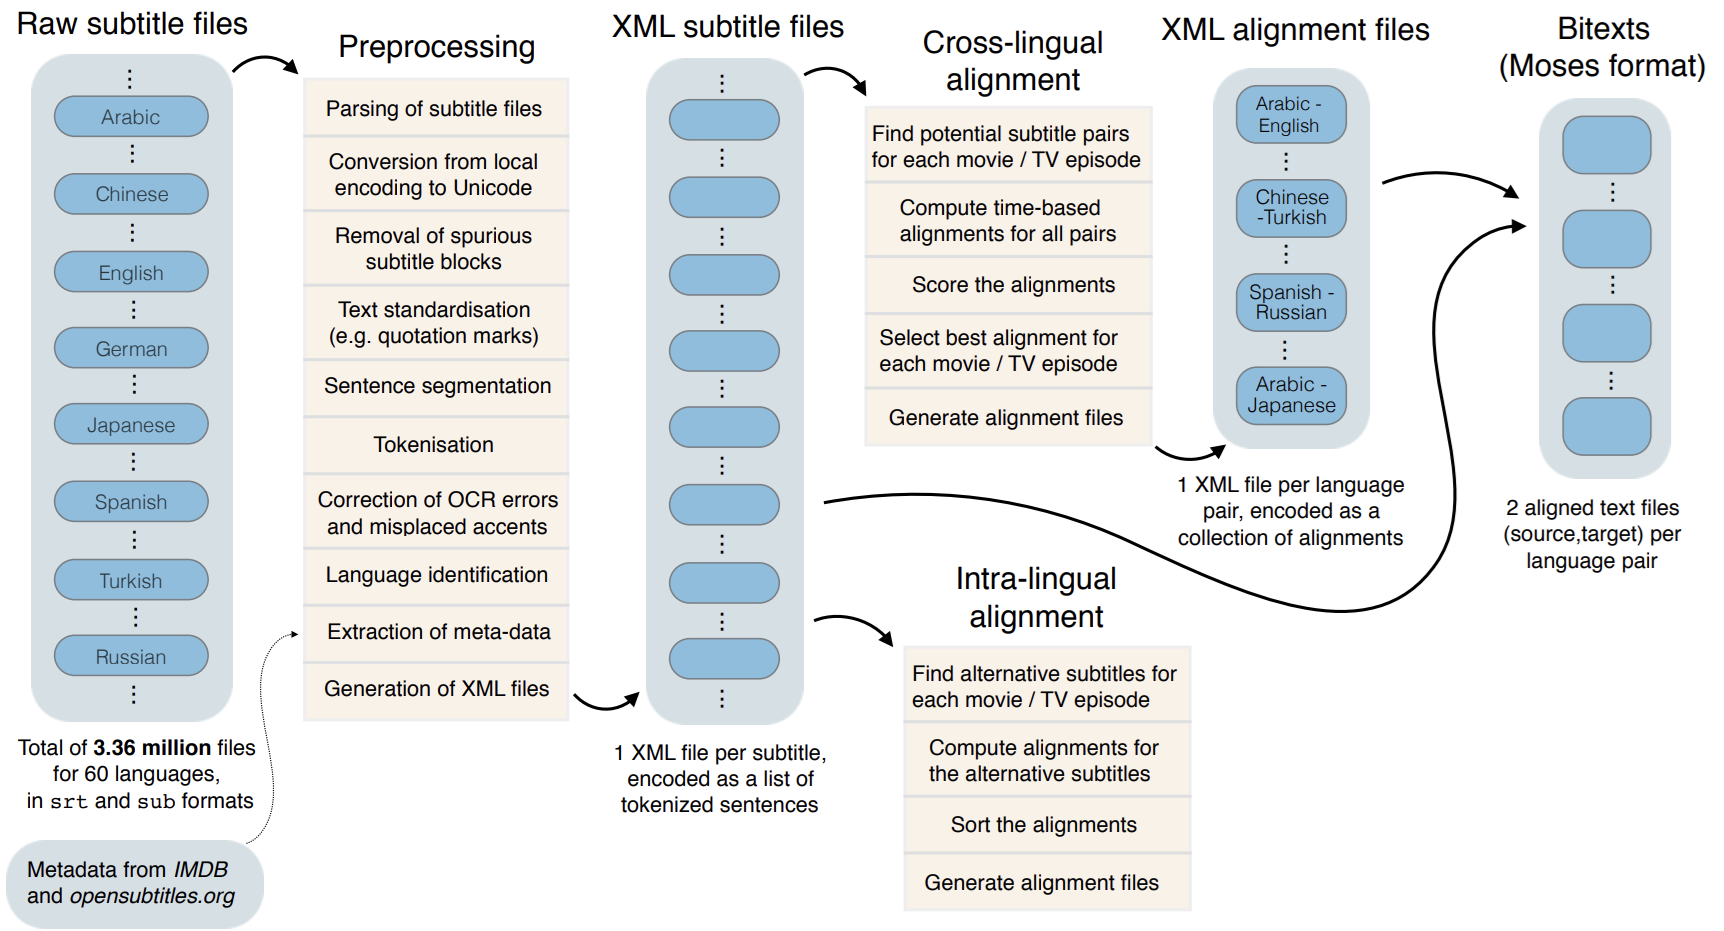
\includegraphics[width=\textwidth]{opensubs_corpus_processing.png}
	\caption{The pipeline producing the OpenSubtitles parallel corpus}
	\label{fig:opensubs pipeline}
\end{figure}

\subsection{Wikipedia}
\contentdescription{{
			\begin{itemize}
				\item advantages: diversity of topics, document level corpus which is not copyrighted, regularly updates dumps
				\item disadvantages: language is technical, does not resemble spoken conversation
				\item describe grouping intro multiple scope corpora: describe category structure of Wikipedia
			\end{itemize}
		}}


Wikipedia offers a large amount of data which can be downloaded in the form of dumps at \url{https://dumps.wikimedia.org/}.
In this work, these dumps are useful in modeling various linguistic contexts that a language learner might be interested in.

\paragraph{Advantages:}
Wikipedia is a valuable resource for several reasons:
It contains a vast number of articles, from a diverse set of topics.
Wikipedia articles have categories assigned to them, which we can use to group articles into linguistic contexts.
This means we do not have to assign the articles to topics ourselves, thus enabling the creation of many smaller-scope corpora from Wikipedia with minimal effort.
The characteristics of the article category system on Wikipedia is discussed in the paragraph below.

Another upshot of Wikipedia is that its articles are licensed under the Creative Commons Attribution-ShareAlike 4.0 International License (\textit{CC BY-SA}).
Because of this, Wikipedia can provide dumps of its entire article database ready for download, with the articles in continuous form and with category metadata attached to them.
This enables us to use the articles as a source for Next Sentence Prediction NSP task.

\paragraph{Disadvantages:}
While Wikipedia offers a large diversity of articles and article topics, the language of the articles follows an academic style of writing.
Thus, the diversity in registers is comparatively low:
Wikipedia is less likely to contain informal language, such as nonstandard language (English: \textit{ain't}, \textit{y'all}) and slang.

Furthermore, it features little language taking conversational form.
% This means that e.g., for English, the second person pronoun "you" occurs very infrequently on Wikipedia. \tocite{Wikipedia rank of you}
This is especially relevant for languages where the certain grammatical forms signify something about the relationship between the speaker and listener:
In Japanese, there exist various linguistic markers of politeness (\textit{Teineigo} and \textit{Keigo}) which play a crucial role in in-person interactions between Japanese speakers, as their presence or absence can signify respect, familiarity or humility with regard to one's interlocutor.
However, such forms are rarely found on Wikipedia, as it does not take the form of a person addressing another person or persons.
Thus, we can see that texts on Wikipedia are of limited use to model linguistic contexts involving in-person conversion.

With these advantages and disadvantages in mind, this work uses Wikipedia articles and their associated metadata to make corpora of various sizes, as explained in the next section.

\paragraph{Modeling Linguistic Contexts:}

One of the chief advantages of Wikipedia as a corpus its diversity of covered topics.
A language learner who is interested in a particular topic will likely find a matching article category on Wikipedia:
For example, a person with an interest in American cinema who is learning English could likely take vocabulary from the articles of the category "20th-century American actresses" to boost their language learning in that linguistic context.
For this reason, we use a number of manually selected categories as testing grounds for our list generation approach.
For each category, we use a number of articles to make a list, then use different articles from the same category as testing data in the evaluation.
We can thus check if learning vocabulary from a category genuinely prepares a learner in understanding texts from that context.

At the same time, a learner could also wish to make a vocabulary list from concrete Wikipedia articles they would like to read.
For that reason, also use single articles as corpora to be processed by our list generation approach.
In that case, no split of training and test data is necessary, as the aim is not to model general knowledge about a domain, but equip the learner with vocabulary about the \textbf{closed} context of a Wikipedia article.
Therefore, in the single-article approach, both the list generation and evaluation use all lines of the article.


% \paragraph{Wikipedia's Category System for Articles}
% There are x categoris on Wikipedia.
% Each article may belong to one or more categories.
% One category can have 0:n parent categories, 0:n child categories.
% Categories therefore not not follow a tree structure, thus most articles belong to more than one top-level category.


\paragraph{Pre-Processing:}
In order to use Wikipedia articles as inputs to our word utility extraction approach, we perform pre-processing on the raw data to filter out source code, as well as chapters that we do not consider to be part of the article text.
This section shortly describes this process.

In their raw form, Wikipedia dumps are written in a markup language called \textit{WikiCode}.
To filter this code and obtain only natural language, we employ the \textit{mwparserfromhell} package \footnote{\url{https://github.com/earwig/mwparserfromhell}} to first strip the text of hyperlinks and markup, and also manually remove metadata such as article categories from the article text.
Next, we filter out the text those sections under headings from a hard-coded list.
This list was compiled by the author and can be seen in Table \ref{tbl:wikipedia-ignored-headings}.
The reason for their exclusion is that these chapters are pure lists which do not contain full sentences, and thus unlikely to contribute to modeling a linguistic context.

\begin{table}[H]
	\centering
	\begin{tabular}{|l|}
		\hline
		\textbf{Section Titles} \\
		\hline
		References              \\
		See also                \\
		External links          \\
		Further reading         \\
		Notes                   \\
		Bibliography            \\
		Filmography             \\
		Discography             \\
		Published works         \\
		Sources                 \\
		Citations               \\
		\hline
	\end{tabular}
	\caption{Common non-article sections in Wikipedia articles}
	\label{tbl:wikipedia-ignored-headings}
\end{table}

Finally, we split the article into individual sentences with the \textit{NLTK} python library \footnote{\url{https://www.nltk.org/}}.
Which these pre-processing steps, we attain a corpus which mostly contains full	sentences which describe the article's topic.


\subsection{Construction of NSP Corpora}
As mentioned in Section {sec:document-level-corpus}, the Next Sentence Prediction task requires consecutive sentences in order to be performed.
Out of the two context-specific corpus types which we employ, only Wikipedia articles consist of such consecutive sentences.
This is confirmed by the fact that preliminary investigations showed that the NSP model's performance on OpenSubs corpora was essentially equal to that of random guessing.
Thus, the NSP task is only performed on Wikipedia articles.
The NSP corpus of an article is constructed by simply taking each consecutive sentence pair from the article, constituting an input datum for the NSP model with an \texttt{is\_next} label of \texttt{True}.
We do not construct negative examples, for the reason that the most words with the most impact on the performance of the model would be words that tell the model that two sentences are \textit{not} connected, which does not appear to us to be useful information.

\subsection{Corpus Characteristics}
We have described the sources of the corpora used in the implementation of our approach, but to gain a better understanding of the data, Table \ref{tbl:corpus-sizes} shows a few key metrics of each corpus type.
It can readily be seen that, while the corpora taken from the OpenSubs subtitles are composed of more lines on average, the Wikipedia articles feature much longer sentences (over three times longer on average than the sentences in subtitles).
This makes sense, as Wikipedia articles are written in an academic style, while movie subtitles tend to be more informal.
Wikipedia articles also contain a higher number of unique words on average, despite containing a lower number of words in total.
This may hint at a higher diversity of vocabulary employed in articles, although a higher number of named entities may also contribute to the higher count of unique words.

\begin{table}[ht]
	\centering
	\begin{tabular}{lrrrrr}
\toprule
 & Corpora & Avg. lines & Avg. words & Avg. unique words & Avg. words per line \\
Corpus Type &  &  &  &  &  \\
\midrule
Wikipedia article & 210 & 253 & 4382 & 1211 & 17.3 \\
OpenSubs subtitle & 632 & 901 & 5436 & 1050 & 6.0 \\
\bottomrule
\end{tabular}

	\caption{General statistics on corpora, per corpus type.}
	\label{tbl:corpus-sizes}
\end{table}


For a more granular overview, we also show these metrics for individual categories in Table \ref{tbl:corpus-sizes-per-wiki-category}.
Most obvious is the fact that the articles of World War II political leaders are, on average, much longer than those films or actors of either gender.
Another notable pattern is that the articles of male actors tend to be longer than those of their female counterparts.


\begin{table}[ht]
	\centering
	\begin{tabular}{lrrrrr}
\toprule
 & \# Corpora & Lines & Words & Unique Words & Words per Line \\
Wikipedia Category &  &  &  &  &  \\
\midrule
1980s English-language films & 26 & 160 & 2950 & 1014 & 18.4 \\
20th-century American actresses & 55 & 188 & 3296 & 934 & 17.5 \\
20th-century American male actors & 108 & 245 & 4157 & 1180 & 17.0 \\
World War II political leaders & 21 & 575 & 10159 & 2340 & 17.7 \\
\bottomrule
\end{tabular}

	\caption{General statistics on corpora, per Wikipedia article category.}
	\label{tbl:corpus-sizes-per-wiki-category}
\end{table}

\section{XAI Methods} \label{sec:xai-methods}
In order to appraise the influence of words in a corpus on the performance of the AI model performing and NLP task, this work employs Explainable AI methods, as explained in Section \ref{sec:xai-as-tools-of-analysis}.

\subsection{Desiderata}
Section \ref{sec:explainable-ai} has explained the use of XAI and stated what kind of XAI methods are especially appropriate for our purpose:
We employ local, feature attribution XAI methods of both model-specific and model-agnostic type, as these allow use to gauge the importance of words in the input from multiple points of view.
Model-specific methods have an advantage in that they typically do not require many model calls to attribute importances to features, and take the model structure into account.
On the other hand, model-agnostic methods are useful in that they can be used on any model and gauge the input-output relationship by performing actual experiments on the model, by observing the way changes to input change the output of the model.

In addition to these taxonomic specifications, an ideal XAI method for word extraction should be both accurate in its feature attributions and should not require extensive computation.
Apart from the benefit of attaining faster results, a computationally lightweight approach allows the model to process more data in less time, presumably boosting the accuracy of the resulting utility evaluation.

There is one further desideratum which we impose for XAI methods:
The XAI method should allow for processing the input sentences in its original form and not, as is common with many XAI methods, as a \textit{bag of words}:
Some methods, such as SHAP and LIME \missingcitation{SHAP, LIME}, can only operate on tasks with a fixed number of features.
When they are employed to explain the decisions of AI models taking whose input is in text format, the words of the sentences are first converted to vector form and provided as mutually independent vectors the model, destroying the information of word order and thus of syntactic relations between words.
This may lead the methods to attribute low importance to words such as "not", which only have an effect in combination with other words.
For this reason, we did not employ popular XAI methods SHAP and LIME in this work.

In the following sections, we propose several concrete XAI methods for use with the described list generation approach.
The relationship of the XAI methods to the NLP tasks are also discussed, as not every combination of XAI method - NLP task is feasible, either because of unrealistic amount of computation or because the results of the combination are difficult to evaluate.
The results of the experiments with these methods is presented in Chapter \ref{ch:evaluation}.

\subsection{Model-Agnostic Approaches}
This section introduces three model-agnostic XAI methods which we used in the implementation to generate vocabulary lists:
All of them work by perturbing the inputs to the model and analyzing the changes in output.
The difference between them is how the perturbation is done:
Single Token Ablation removes single tokens from the inputs, whereas Single Token Summary works by setting the input to a single token.
The third method, Progressive Summary, attempts to find the most important words in sentences by iteratively building up the input sentence, one token at a time.

\subsubsection{Single Token Ablation}
Our aim in using XAI methods is to find out which words, if known, improve the model's performance the most, when compared to not knowing the word.
Perhaps the simplest way of testing this is by going through every word in the input to the AI model, and checking the model performance when the word is removed from the input.
Within this work, this approach is called \textbf{Single Token Ablation}.

\paragraph{Approach:}
Given an input line or a pair of lines:
For each word in the input, create a variation of the input where the word is removed.
Run the model on all inputs and measure how much performance is degraded in each case.
Estimated utility is the difference in performance between not removing and removing the word.

\paragraph{Advantages:}
One advantage of Single Token Ablation is its conceptual simplicity, as it is very easy to implement.
Furthermore, its time complexity is fairly minimal for a feature method, as it requires only one model call for each unique token in the sentence ($\mathcal{O}(n)$).

\paragraph{Disadvantages:}
The main downside of this method is that, in long sentences, leaving out a single token does not change the meaning of the sentence to such an extent that the sentence becomes unintelligible.
Assuming the AI model can process sentences with missing words with similar accuracy as humans, the impact on performance may therefore be minimal or not predictive of actual usefulness.
Furthermore, this method does not take into account the utility of a word in the context of word combinations.

\paragraph{Summary:}
Among model-agnostic methods, Single Token Ablation is a computationally inexpensive whose feature perturbation consists of ablating single words.
We may think of this method as simulating a language learner who already knows all words in a sentence except for one, and as such it may not model word utility in such a way that the resulting list is useful for beginners.

\subsubsection{Progressive Summary}
While Single Token Ablation is easy to implement and cheap to execute, its downside is that the performance differences may not be representative of actual utility.
To achieve a more accurate evaluation, we may think of an approach that is in some sense the inverse of removing single words from sentences:
Checking which words are the most essential by reducing the sentence a minimal number of words.

\paragraph{Approach:}
Given an input line, we first let the AI model run on the unaltered input.
We then go through every word in the input line, let the model run with the single word as input, and check which of the words produces an output that is close to the output for the unaltered line.
We can thus see which word summarized the sentence the best.

However, we need not stop here:
After determining the most essential word in the sentence, we can check which words from the remaining pool of words brings the outputs closer still.
By iterating this method, we progressively reconstruct the original sentence, which each step being the best next word to add in order to restore the original output.
For this reason, we refer to this method as \textbf{Progressive Summary}.
Here, the estimated utility of a word is the boost in performance which is brought to the sentence when the word is added.

\paragraph{Advantages:}
The Progressive Summary approach models the perception of a beginner-level language learner better than Single Token Ablation.
The latter asks which single word, when lacking, degrades performance the most.
Progressive Summary instead asks which words, if known, bring language performance closest to knowing all words in the sentence.

\paragraph{Disadvantages:}
Progressive Summary is much more computationally intensive than Single Token Ablation, which requires only one model call per word in the sentence.
Because of its iterative approach, for a sentence with 10 words, Progressive Summary calls the model $10+9+8+... $ or $\sum_{i=1}^{n}i = \frac{n^2 + n}{2}$ times, which is a time complexity of $\mathcal{O}(n^2)$.


\paragraph{Compatibility with NLP tasks}
As Progressive Summary starts from a set of one words and then progresses to larger sets, it is difficulty to meaningfully employ in combination with an NLP task whose input is not a single line, e.g., Next Sentence Prediction.
One could circumvent the issue by leaving one of the sentences in its original form and only perturbing the other, but this can hardly be seen as a modeling of natural language ability.

\todo{Maybe: Describe issues of using PS with models whose output is single number: Approximating with single words may not be meaningful approximation at all. But should test empirically.}

As such, our implementation Progressive Summary is not used with Next Sentence Prediction.

\paragraph{Summary:}
Progressive Summary attempts to find the most important words in a sentence one by one, by first reducing the sentence to one word, then two etc., and using a distance metric to compare the "summaries" to the original sentence.
The words which bring the model output for the summary closest to that of the original sentence are regarded as the most useful.

\subsection{Model-Specific Methods}
The model-agnostic methods so far are general tools which can be employed on any model.
However, as many of the latest state-of-the-art AI models follow the Neural Network architecture, and more specifically the transformer architecture (see Section \ref{sec:transformer}), we also attempt word utility estimation with methods specific to these model.
These model-specific XAI methods have the advantage of being computationally efficient:
Model-agnostic methods extract information about the model by perturbing its inputs and analyzing the resulting changes in the output.
This requires many model calls for one input datum.
In contrast, model-specific methods can analyze the input-output relationship with only one model call, as they look into the model itself for information.
We therefore try two model-specific methods for analyzing word utility as well, as their more efficient calculations means they can process more input data in a given time, which should increase the accuracy of the resulting word list.
\todo{Correction relevance propagation is no longer employed}

\subsubsection{Attention as Explanation}
One XAI method which has been proposed to explain the decision of transformer models specifically is the transformer's own attention mechanism:
As stated in Section \ref{sec:transformer}, transformer model (if their input is in text format) use self-attention to assign importance to the connections between tokens in the input.
This may be used as a kind of explanation, as words which have strong connections to many words in the sentences presumably are more important than those receiving less self-attention.

An important difference to the model-agnostic methods explained before is that we do not control word masking with a tokenizer \textit{independent of the model}, thus the splitting of words is not under our direct control.
The tokenizers used are \texttt{bert-base-uncased} and \texttt{sentence-transformers/paraphrase-MiniLM-L6-v2}.
These produce tokens on a sub-word level, which means that we must perform post-processing on the attentions to acquire values on the word level and make vocabulary lists than contain full words.
For BERT tokens, this is a simple process as sub-tokens which are not at the beginning of a word start with "\#\#".
\todo{Insert sub-word tokenization example from BERT}
The estimated utility for the reconstructed token is calculated by taking the sum of the attention values of each sub-token.

\paragraph{Approach:}
A transformer model is run with one line as input.
The transformer outputs an attention tensor, which attributes a value to each pair of tokens in the input (this includes special tokens from the tokenizer, such as and \texttt{[SEP]} and punctuation).
We then aggregate the attention of each token by summing over one axis of the attention tensor of all connections each token has, and over all the attention heads, resulting in one scalar value per token.
The original tokens of the tokenizer are merged
Next, special tokens and punctuation are filtered
Finally, we normalize the attentions such that the attention for all words in the line sums up to one.
The attributed attention to a word is its estimated utility.

\paragraph{Advantages:}
As hinted at before, this method uses one model call for one input line, and thus has a time complexity of $\mathcal{O}(1)$.

\paragraph{Disadvantages:}
One disadvantage of Attention as our attention mechanism is that attentions are attributed to input tokens of the model.
Unlike the model-agnostic methods where word masking is controlled by a tokenizer \textit{independent of the model}, the tokenizer cannot be changed.
AI models are trained with some tokenizer as preprocessing the input, and this tokenizer cannot be changed, lest we change the input format to the AI model itself.
This is an issue because it means that lists generated with the model-specific tokenizer are not necessarily comparable to lists from model-agnostic methods, as the tokenization method may differ.

In addition to this technical downside, Attention is controversial as a mechanism to explain model decisions.
\tocite{Attention is not Explanation}

\paragraph{Summary:}
Among the XAI methods used in this work, Attention as Explanation requires the least resources, and it is not restricted to any one NLP task (although the model must be of transformer type).
However, we do not control the tokenizer used directly.
While the NSP model uses the same tokenizer that is also used for token masking in the model-agnostic XAI methods, the sentences embedding model uses a different tokenizer.



% \subsubsection{Layer-wise Relevance Propagation (not yet implemented $\rightarrow$ may be deleted)}
% \paragraph{Approach:}
% \paragraph{Advantages:}
% \paragraph{Disadvantages:}
% \paragraph{Summary:}
%
%
\section{Implementation with Chosen NLP Tasks, Corpora, and XAI Methods} \label{sec:implementation-final}
The previous chapters have argues for the choice of components in our theoretical approach to vocabulary list generation and evaluation. 
This final section about our implementation describes how the chosen components interact in our implementation.

\contentdescription{
	Describe which comps are compatible, and where it is not obvious, how exactly they are made to work with each other.
}
